%!TEX root = ../project.tex
\part{Analysis}
\iffalse
\begin{description}
	\item[What is your idea?] \hfill \\
		A program to help visualize the orbits of planets and satellites
	\item[Is your idea complex enough?] \hfill \\
		It will require a lot of complex equations to calculate the
		positions of each object at any given time, and the use of
		graphics libraries to display the objects.
	\item[Who is your user?] \hfill \\
		My end user is Dr.~Naylor (dnaylor@kefw.org). I have not yet
		decided whether to aim it towards use in front of a class, or
		for the students to use themselves.
	\item[What programming languages do you know?] \hfill \\
		My main language is C, but I also know some Python and I am
		currently learning some Common Lisp. I plan to write the program
		mainly in C because of its good performance and compatibility
		with many external libraries. I might try to include some Lisp
		in as well.
	\item[Do you need to use a database or other data stored?] \hfill \\
		I don't think I will require any large databasing tool like SQL,
		but I might have external files for storing information about
		planets.
	\item[What do you need to learn?] \hfill \\
		I will need to learn how to use the external libraries that I
		intend to use for graphics. I plan on using either OpenGL or
		SDL.
	\item[What websites and books can help you?] \hfill \\
		Wikipedia will be very useful for finding figures like the mass
		of a planet. I have a copy of \emph{The C Programming Language}
		by Dennis Ritchie and Brian Kernighan, which I use as a
		reference while I am programming in C.
		\\
\end{description}
\fi
\section{Investigation}
\iffalse
\subsection{Background}

King Edward VI Five Ways school teaches Astronomy at GCSE level. One part of the
coarse involves understanding the orbits of planets. It is very hard to
visualize without some sort of animation to help. At the moment they use a basic
web applet, with minimal features.
\fi
\subsection{Problem}
Dr.~Naylor, who teaches astronomy, needs a way to help his students visualise
the orbits of the planets to help them to understand Kepler's laws. 

\subsection{Current Solution}
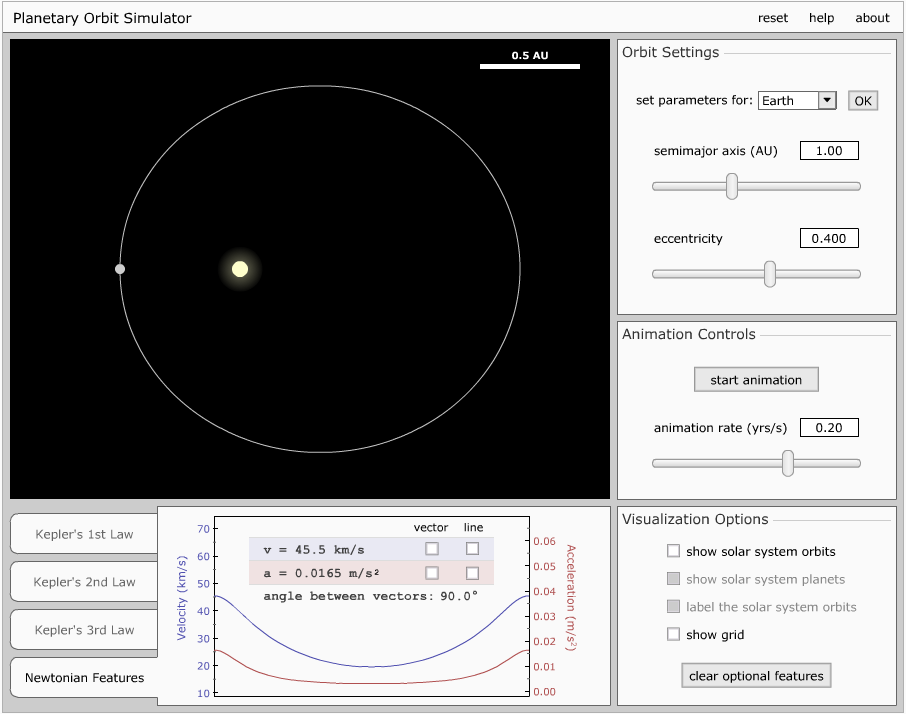
\includegraphics[width=\textwidth]{./img/existing-solution.png}

The current system shows the solar system in 2 dimensions. It only shows one
planet by default but there is the option to show the others. It only allows one
planet's properties to be manipulated at a time, and the properties that can be
changed are the semimajor axis and eccentricity (and these can be set to the
values of a real planet using the drop-down menu). The animation speed can also
be adjusted. The program has strict limits to what values these parameters can
be set to. The strength of this solution is its visualisations of Kepler's laws,
which is what the end user really needs from the program.

\subsection{Prospective Users}
My main user will be Dr.~Naylor, as he is the
astronomy teacher at my school. He would like to be able to stand in front of a
class and use the program to help the students visualise Kepler's laws while he
explains them. It may also be useful if the program can be used by the students
in their own time, if they didn't understand something in the lesson. I would
also like to allow the student to experiment with as I think it would make them
more interested. Dr.~Naylor isn't very computer literate, so the interface
should be easy to understand. Also if I'm aiming to have the students use it do
there will be a wide variety of abilities. 


\subsection{User's Needs and Limitations} 

